%Terminal Command = xelatex -pdf FileName
%Pretreatment ========================================================
\documentclass{beamer}
\mode<presentation> {
\usetheme{Madrid}
}

\usepackage{graphicx}
\usepackage{booktabs} 
\usepackage{lingmacros}
\usepackage{tree-dvips}
\usepackage{hyperref}
\usepackage{amsmath}
\usepackage{amssymb}
\usepackage{multicol}
\usepackage{geometry}
\usepackage{listings} 
\usepackage{verbatim}
\usepackage{cite}
\usepackage{algpseudocode}
\usepackage{algorithm}
\usepackage{listings} 
\usepackage{verbatim}
\usepackage{subfigure}
\usepackage{appendix}  
\usepackage{graphics}
\usepackage{color}

%Infomation ========================================================
\title[Fast Hog]{Pedestrian Detection in Small Device with Fast Hog and Cluster}
\author{Kazuki Amakawa}
\institute[USTB MPA]
{
University of Science and Technology Beijing, Mathematics and Physicis Academy
\medskip\\
\textit{KazukiAmakawa@gmail.com}
}
\date{\today}

%Title and menu ========================================================
\begin{document}

\begin{frame}
\titlepage
\end{frame}

\begin{frame}
\frametitle{Overview} 
\tableofcontents
\end{frame}

%Main ========================================================
%Section ========================================================
\section{Introduction}
\subsection{Pedestrian Detection}
\begin{frame}
\textbf{Pedestrian Detection}
\end{frame}



\begin{frame}
\frametitle{Introdution 1}
\textbf{What is Pedestrian Detection?}
\\Pedestrian detection is an essential and significant task in any intelligent video surveillance system, as it provides the fundamental information for semantic understanding of the video footages. It has an obvious extension to automotive applications due to the potential for improving safety systems. 
\\[2ex]
\textbf{Usage}
\\1) Autonomous vehicles
\\2) Surveillance camera early-warning
\\3) Robort vision in Pedestrian Detection
\\4) Pertreatment of Pedestrian re-identification (re-id)
\\5) Motion analysis
\\...
\\[2ex]
\end{frame}



\begin{frame}
\frametitle{Introdution 2}
\textbf{Object Detection}
\\1) Pre-treatment of image
\\2) Get the regions may include object
\\3) Describing these regions
\\4) Clasify all description
\\5) Determine the region which include object
\\[2ex]
In Pedestrian Detection problem, we aim at pedestrain. So the object above is equal to pedestrain. And we have the processing of perdestrain detection
\\[2ex]
\textbf{Pedestrian Detection}
\\1) Pre-treatment of image
\\2) Extracting candidate regions may include human (or just include object)
\\3) Describing these region(or object)
\\4) Clasify all description
\\5) Find pedestrain
\end{frame}



\begin{frame}
\frametitle{Introdution 3}
Feature: include edge, texture, color and motion\\[2ex]
\textbf{Human Detection Feature}\cite[Nguyen2016]
\\1) Shape features (pixel level edge-based features)
\\Disadvantage: Noisy, Pose-specific\\[1ex] 
2) Region lever edge-based features (Hog)
\\Disadvantage: Need large calculation, high dimension(difficult for classification)
\\Pre-processing, PCA, Gabor filter bank(not understant)\\[2ex]
3) DNN Feature
\end{frame}



\begin{frame}
\frametitle{Introdution 4}
\textbf{Classification}
\\Processing:  TrainData -> Train -> Model <- TestData\\
\ \ \ \ \ \ \ \ \ \ \ \ \ \ \ \ \ \ \ \ \ \ \ \ \ \ \ \ \ \ \ \ \ \ \ \ \ \ \ \ \ \ \ \ \ \ \ \ \ \ |\\
\ \ \ \ \ \ \ \ \ \ \ \ \ \ \ \ \ \ \ \ \ \ \ \ \ \ \ \ \ \ \ \ \ \ \ \ \ \ \ \ \ Classification
\\Method: SVM(PL-SVM, linearSVM), AdaBoost, DNN(softmax ...)
\\SVM: Small model and easy control
\end{frame}





\subsection{Pedestrian Detection in small device}
\begin{frame}
\textbf{Pedestrain detection in small device with fish eye camera}
\end{frame}



\begin{frame}
\frametitle{Introdution 5}
\textbf{Notice of Pedestrian detection in surveillance camera and early-earning system}
\\1) Continuous images, different from normal image pedestrian detection, surveillance have less moving and it is easy to determine the background and object
\\2) Realtime processing, in our project, we have to process one image in less than 1 second
\\3) Bad enviroment: Natural influence: rain, windy; Human influence: too many object; Noisy
\end{frame}



\begin{frame}
\frametitle{Introdution 6}
\textbf{Problem in small device}
\\Less memory and CPU speed, so it is not easy to run a DNN network on these devices
\\[2ex]

\textbf{Problem in fish eye camera}
\\1) Distort Image, so other elder model may cannot be used
\\2) Infrared Model, bad image quality, Noisy
\\[2ex]
Also, as human structure is different from normal object structure, it have more motion and edge. So it is not easy to build the model.
\end{frame}



\begin{frame}
\frametitle{Introdution 7}
\textbf{Shortage of traditional Pedestrian detection method}
\\High time complex (Hog)
\\[2ex]
\textbf{Shortage of DNN Pedestrian detection method}
\\1) Model too large
\\2) Cannot find C code project
\\3) Need more train data
\end{frame}





%Section ========================================================
\section{Related Work}
\begin{frame}
\textbf{Related Work}
\end{frame}



\begin{frame}
\thispagestyle{empty}
%\frametitle{Related Work - Main}
\begin{figure}[H]
\centering
\begin{minipage}[b]{0.9\textheight}
\includegraphics[width=0.95\textwidth]{Figure/mainalgo.png}
\end{minipage}
\caption{Fast Hog main processing}
\end{figure}
\end{frame}



\subsection{Get the object: Pretreatment}
\begin{frame}
\frametitle{Get the object: Pretreatment}
\begin{figure}[H]
\centering
\subfigure[Old Image]{
\begin{minipage}[b]{0.46\textwidth}
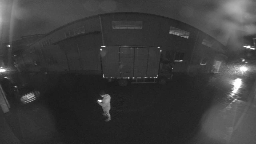
\includegraphics[width=1\textwidth]{Figure/Pretreatment/Img1.png}
\end{minipage}
}
\subfigure[New Image]{
\begin{minipage}[b]{0.46\textwidth}
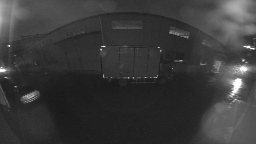
\includegraphics[width=1\textwidth]{Figure/Pretreatment/Img2.png}
\end{minipage}
}
\subfigure[Result]{
\begin{minipage}[b]{0.46\textwidth}
\includegraphics[width=1\textwidth]{Figure/Pretreatment/Result.png}
\end{minipage}
}
\caption{Negative two images}
\end{figure}
(Parameter: NegThs = 10)
\end{frame}



\subsection{Get the object: DBSCAN}
\begin{frame}
\thispagestyle{empty}
\textbf{DBSCAN Principle}\\
\footnotesize
A point $p$ is a inner point if at least $minPts$ points are within distance $\epsilon$.\\
A point $q$ is directly reachable from $p$ if point $q$ is within distance $\epsilon$ from point $p$ and $p$ must be a inner point.\\
A point $q$ is reachable from $p$ if there is a path $p_1, \ldots, p_n $with $p_1 = p$ and $p_n = q$, where each $p_{i+1}$ is directly reachable from $p_i$.\\
All points not reachable from any other point are outliers.\\
Now if $p$ is a core point, then it forms a cluster together with all points that are reachable from it. Each cluster contains at least one core point; non-core points can be part of a cluster, but they form its "edge", since they cannot be used to reach more points.

\begin{figure}[H]
\centering
\subfigure[Algorithm]{
\begin{minipage}[b]{0.46\textwidth}
\includegraphics[width=1\textwidth]{Figure/DBSCAN/Algorithm.png}
\end{minipage}
}
\subfigure[Cluster method]{
\begin{minipage}[b]{0.46\textwidth}
\includegraphics[width=1\textwidth]{Figure/DBSCAN/Processing.png}
\end{minipage}
}
\caption{DBSCAN}
\end{figure}

\end{frame}



\begin{frame}
\frametitle{Related Work - Get the object: DBSCAN}
\textbf{Result}
\begin{figure}[H]
\centering
\subfigure[Differential Image]{
\begin{minipage}[b]{0.46\textwidth}
\includegraphics[width=1\textwidth]{Figure/DBSCAN/InpImg.png}
\end{minipage}
}
\subfigure[Cluster Image]{
\begin{minipage}[b]{0.46\textwidth}
\includegraphics[width=1\textwidth]{Figure/DBSCAN/Result.png}
\end{minipage}
}
\caption{DBSCAN}
\end{figure}

\textbf{Advantage}
Less Noisy, Fast, Needn't care about $k$ in K-means
\end{frame}



\subsection{Get the feature: Hog Descriptor}
\begin{frame}
\thispagestyle{empty}
%\frametitle{Related Work - Get the feature: Hog Descriptor}
\footnotesize
\begin{algorithm}[H]
\caption{Hog Descriptor}
\begin{algorithmic}
\State Input: $Image[Oriheight][Oriwidth]$
\State STEP1: Down Sample $Image = resize(Image, (height, width))$
\State STEP2: Gamma transform: $Image[i][j] = GammaTable[Image[i][j]]$
\State STEP3: Get the $Gradient$ and $Angle$ image with Sobel operator
\State STEP4: $BlockImgs = [Block\ New\ Image\ with\ BlockX, BlockY, StrideX, StrideY]$
\For {Block in BlockImgs}
\State $Cells = [Get\ the\ Cell\ with\ CellX, CellY in every Block]$
\For {Cell in CellImgs}
\State Statistic Histogram of gradient Hisrogram[nbins]
\State Normalize the Hisrogram
\EndFor
\State Get the $Hog\ descriptor\ in\ the\ Block$
\EndFor
\State Output: $Hog\ descriptor\ of\ the\ image$

\end{algorithmic}
\end{algorithm}
\end{frame}


\begin{frame}
\frametitle{Details of Hog}
\textbf{Gamma Transform}
\begin{displaymath}
Img_{output} = A\cdot Img_{Input}^{\gamma}
\end{displaymath}
(Parameter Gamma = 0.5)\\[3ex]
\textbf{Gradient and Angle}
\begin{displaymath}
SobelX = [-1, 0, 1]\ \ \ \ SobelY = [-1, 0, 1]^{T}
\end{displaymath}
Convolution
\begin{displaymath}
GradientX = Image \ast SobelX
\end{displaymath}
\begin{displaymath}
GradientY = Image \ast SobelY
\end{displaymath}
So we have 
\begin{displaymath}
Gradient = \sqrt{GradientX^2 + GradientY^2}
\end{displaymath}
\begin{displaymath}
Angle = \arctan\left[GradientY \over GradientX\right]
\end{displaymath}
\end{frame}



\begin{frame}
\thispagestyle{empty}
\begin{multicols}{2}
\begin{figure}[H]
\centering
\subfigure[Block X]{
\begin{minipage}[b]{0.4\textheight}
\includegraphics[width=0.4\textheight]{Figure/Hog/BlockX.png}
\end{minipage}
}
\subfigure[Block Y]{
\begin{minipage}[b]{0.4\textheight}
\includegraphics[width=0.4\textheight]{Figure/Hog/BlockY.png}
\end{minipage}
}
\subfigure[Statistic Data]{
\begin{minipage}[b]{0.5\textheight}
\includegraphics[width=0.5\textheight]{Figure/Hog/Statistic.png}
\end{minipage}
}

\subfigure[Cells from block]{
\begin{minipage}[b]{0.3\textheight}
\includegraphics[width=0.3\textheight]{Figure/Hog/BlockCell.png}
\end{minipage}
}

\subfigure[A Cell]{
\begin{minipage}[b]{0.4\textheight}
\includegraphics[width=0.4\textheight]{Figure/Hog/Cell.png}
\end{minipage}
}

\caption{Hog Block and Cells}
\end{figure}
\end{multicols}
\end{frame}




\subsection{Classification: SVM}
\begin{frame}
\frametitle{Related Work - Classification: SVM}

\end{frame}





%Section ========================================================
\section{Details and hit of the method}
\subsection{DBSCAN}
\begin{frame}
\frametitle{Details - DBSCAN}
\end{frame}



\subsection{Hog Descriptor}
\begin{frame}
\frametitle{Details - Hog Descriptor}
\end{frame}



\subsection{About Plan A}
\begin{frame}
\frametitle{Related Work - About Plan A}
\end{frame}





%Section ========================================================
\section{IFECP(Infrared Fish Eye Camera Pedestrian Database) database}
\begin{frame}
\frametitle{IFECP Database}
\end{frame}





%Section ========================================================
\section{Result}
\begin{frame}
\frametitle{Result}
\end{frame}





%Section ========================================================
\section{Segmentation in pedestrain detection}
\begin{frame}
\frametitle{Segmentation in pedestrain detection}
\end{frame}




%Section ========================================================
\section{Reference}
\begin{frame}
\bibliographystyle{plain}
\bibliography{/Users/kazukiamakawa/Desktop/お仕事関連/Paper/KazukiAmakawa.bib}
\end{frame}



\end{document}



















